\documentclass[letter]{article}

\usepackage[margin=1in]{geometry} % make more efficient use of the page

\usepackage[utf8]{inputenc}

\usepackage{amsmath} % math tools
\usepackage{amsfonts} % math tools
\RequirePackage{amssymb} % math tools
\RequirePackage{amsbsy} % math tools

\renewcommand{\vec}[1]{\ensuremath{\boldsymbol{#1}}} % make vectors nicer

\usepackage{graphicx} % graphics
\usepackage{xcolor} % colored text

\usepackage{hyperref} % URLs and such
\usepackage{verbatim} % allows \verb-- command

\usepackage{algorithmicx} % algorithm environment
\usepackage{listings} % code listings

\usepackage{natbib} % bibliography


\title{CMDA 3634 \\ Lab 02 Report}
\author{Russell J. Hewett}

\begin{document}

\maketitle

\begin{enumerate}
    \item What command did you run to compile your program?
    % Hint: use \texttt{} for monospaced font
    
    \textbf{ANSWER:} \texttt{gcc -o vector3d vectors.c -lm}

    \item For the scalars $\alpha=0.25$ and $\beta = 0.56$ and vectors,
        \begin{align*}
            \vec{x} = \left[\begin{array}{r} 1.0 \\ 1.5 \\ 2.3 \end{array}\right], \;
            \vec{y} = \left[\begin{array}{r} 0.01 \\ 5 \\ 17.1717 \end{array}\right],
        \end{align*}
        use your program to compute the following values:
        \begin{enumerate}
            \item $m = \lVert\vec{x}\rVert$, the length of $\vec{x}$.
            \item $\vec{z_1} = \alpha * \vec{x} + \vec{y}$, the \texttt{*axpy} operation for 3-vectors.
            \item $\vec{z_2} = \beta * \vec{y} + \vec{y}$, the \texttt{*axpy} operation for 3-vectors.
            \item $a = \left<\vec{x}, \vec{y}\right>$, the inner product of $\vec{x}$ and $\vec{y}$ for 3-vectors.
        \end{enumerate}
        Include a screenshot of the output.  Be sure that your output indicates which question it corresponds to.
    % Hint: use \includegraphics[scale=x]{} to include your image
    
    \textbf{ANSWER:}\\
    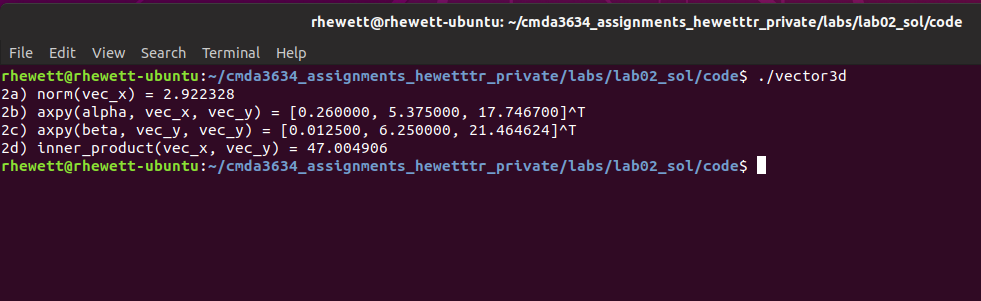
\includegraphics[scale=0.4]{screenshot.png}

    \item Using an un-ordered list, give three (3) advantages we gained by using structures to pass the vector data to our functions.
    % Hint: use \includegraphics[scale=x]{} to include your image
    
    \textbf{ANSWER:}
    \begin{itemize}
        \item Cleaner, easier to read function signatures and code.
        \item Easier future modification of layout of the data type.
        \item Can nest calls, e.g., \texttt{norm(axpy(...))}.
        \item (disadvantage) Extra care to avoid unnecessary copies (pass-by-pointer).
    \end{itemize}

    \item Other than the instructor or TAs, who did you receive assistance from on this assignment?
    
    \textbf{ANSWER:} No one.
\end{enumerate}

% I leave this part commented out as some example code if you need it.
% \section{Introduction}
% There is a theory which states that if ever anyone discovers exactly what the Universe is for and why it is here, it will instantly disappear and be replaced by something even more bizarre and inexplicable.
% There is another theory which states that this has already happened.

% \begin{figure}[h!]
% \centering
% \includegraphics[scale=1.7]{universe}
% \caption{The Universe}
% \label{fig:universe}
% \end{figure}

% \section{Conclusion}
% ``I always thought something was fundamentally wrong with the universe'' \citep{adams1995hitchhiker}

% \bibliographystyle{plain}
% \bibliography{references}
\end{document}
